\documentclass[12pt]{article}

\usepackage{titlesec}
\titleformat
{\section} % command
[display] % shape
{\normalfont\fontsize{14}{14}\sffamily\bfseries} % format
{} % label
{1ex} % sep
{
    \color{cyan}\rule{0.7\textwidth}{6pt}\vspace{2pt}\newline
    \color{black}
} % before-code

\titleformat
{\subsection} % command
[display] % shape
{\normalfont\fontsize{14}{14}\sffamily\bfseries} % format
{} % label
{1ex} % sep
{
    \color{cyan}\rule{0.5\textwidth}{3pt}\vspace{5pt}\newline
    \color{black}\hspace{11pt}
} % before-code
\titlespacing*{\subsection}{0pt}{0ex}{0em}

\setlength{\parskip}{0.5em}

%https://www.latextemplates.com/template/lachaise-assignment

%---DOCUMENT MARGINS---
\usepackage{geometry} % Required for adjusting page dimensions and margins
\geometry{
	paper=a4paper, % Paper size, change to letterpaper for US letter size
	top=4.25cm, % Top margin
	bottom=3cm, % Bottom margin
	left=2.5cm, % Left margin
	right=2.5cm, % Right margin
	headheight=3cm, % Header height
	%footskip=1.5cm, % Space from the bottom margin to the baseline of the footer
	headsep=0.8cm, % Space from the top margin to the baseline of the header
	%showframe, % Uncomment to show how the type block is set on the page
}

\usepackage{cmap}
\usepackage[utf8]{inputenc}
\usepackage[T2A]{fontenc}
\usepackage[bulgarian,english]{babel}

\usepackage{amsmath}
\usepackage{makecell}
\usepackage{tabulary}


\usepackage{indentfirst}

\usepackage{fancyhdr}
\pagestyle{fancy}
%\setlength{\headheight}{35pt}

\usepackage{background}
\backgroundsetup{contents={
\includegraphics[width=28cm,height=3.45cm]{./structure/header_background.png}},scale=1,placement=top,opacity=0.8}

\fancyhead{}
%\fancyhead[L]{
\includegraphics[height=2cm]{ruo.jpg}}
%\fancyhead[R]{
\includegraphics[height=2cm]{sap.png}}

\fancyhead[L]{\begin{minipage}{\textwidth}\flushleft
\includegraphics[width=2.8cm]{./structure/ruo.png} \vspace{10pt} \end{minipage}}
\fancyhead[R]{\begin{minipage}{\textwidth}\flushright
\includegraphics[width=2.8cm]{./structure/sap.png}\end{minipage}}

\fancyhead[C]{\begin{minipage}{\textwidth}\color{white}\centering\small\bf{\fontfamily{cmss}\selectfont
\textit{ОТКРИТО ПЪРВЕНСТВО НА СОФИЯ ПО ИНФОРМАТИКА}\\\
\textit{15 ноември 2021 г.}\\
\textit{Група C, 7–8 клас} \vspace{-10pt}} \end{minipage}}
\renewcommand{\headrulewidth}{0pt}

\fancyheadoffset[L,R]{1.5cm}

\pagenumbering{gobble}

\usepackage{graphicx}
\usepackage{wrapfig}
\sloppy

\begin{document}

\section*{Задача C3. Кули}

Напоследък Алекс доста скучаел, седейки само пред компютъра, и за да преодолее жаждата за сън, решил да си измисли някаква игра, каквато и да е! Първото нещо, което му се мярнало пред погледа, била купчината от $S$ гумички, всяка от които била с форма на куб с размери $1$см$\times1$см$\times1$см. И ето, че идеята веднага се родила. Той искал да ги нареди в редица от кули, така че всяка кула да е съставена от някакъв положителен брой гумички. Също така, всяка кула трябвало да е с височина или строго по-малка от тези на двете ѝ съседни, или строго по-голяма (ако кулата е крайна се гледа само единият ѝ съсед). Разбира се едно такова нареждане е доста лесно за съставяне. На Алекс обаче му било интересно колко са всички възможни начини, по които може да нареди гумичките, така че да е спазено условието. Включете се в неговата кауза срещу скуката, като напишете програма \textbf{towers}, която по даден брой гумички, да намира броя на всички възможни редици от кули от описания вид. Тъй като той може да е доста голям, изведете остатъка му при деление с 1000000007.

На фигурата е показано едно примерно нареждане на 11 гумички в редица от 5 кули.
\begin{center}
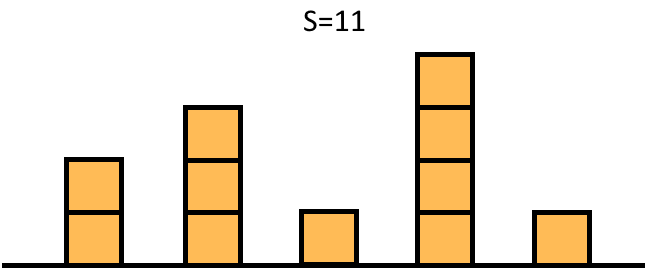
\includegraphics[scale=0.7]{towers_example_1}
\end{center}

\subsection*{Вход}
От единствения ред на стандартния вход се въвежда едно положително число $S$ - броят на гумичките.

\subsection*{Изход}
На един ред изведете едно число - търсения брой начини по модул $10^9+7$.
\\ \\ \\
\subsection*{Ограничения}
$1 \leq S \leq 5000$

\subsection*{Подзадачи}
\begin{table}[hbtp]
\hspace{5pt}
\setlength\extrarowheight{2pt}
\begin{tabulary}{1.0\textwidth}{ |c|c|c| }
\hline
    \textbf{Подзадача} & \textbf{Точки} & $S$ \\
\hline
    1 & 20 & $\leq 10$\\ 
\hline
    2 & 15 & $\leq 40$\\ 
\hline
    3 & 10 & $\leq 100$\\ 
\hline
    4 & 15 & $\leq 500$\\  
\hline
    5 & 30 & $\leq 2000$\\  
\hline
    6 & 10 & $\leq 5000$\\  
\hline
\end{tabulary}
\end{table}
\vspace{-2ex}
\indent \textit{Точките за подзадача се получават само ако се преминат всички тестове предвидени за нея.}

\subsection*{Пример}
\begin{table}[hbtp]
\hspace{5pt}
\setlength\extrarowheight{2pt}
\begin{tabulary}{1.0\textwidth}{ |l|l|l| }
\hline
    \textbf{Вход} & \textbf{Изход} & \textbf{Обяснение на примера} \\
\hline
    \makecell[tl]{6} & 
    \makecell[tl]{12} & 
    \makecell[tl]{Всички възможни редици са: \\
    $\{1,2,1,2\}$ $\{2,1,2,1\}$ $\{1,3,2\}$ $\{2,1,3\}$ $\{2,3,1\}$ \\
    $\{3,1,2\}$ $\{1,4,1\}$ $\{2,4\}$ $\{4,2\}$ $\{1,5\}$ $\{5,1\}$ $\{6\}$} \\
\hline
    \makecell[tl]{20} & 
    \makecell[tl]{6949} & 
    \\
\hline
\end{tabulary}
\end{table}
	
\end{document}






